\documentclass[tikz, border=15pt]{standalone}
\usepackage{amsmath}
\usepackage{xcolor}

\begin{document}

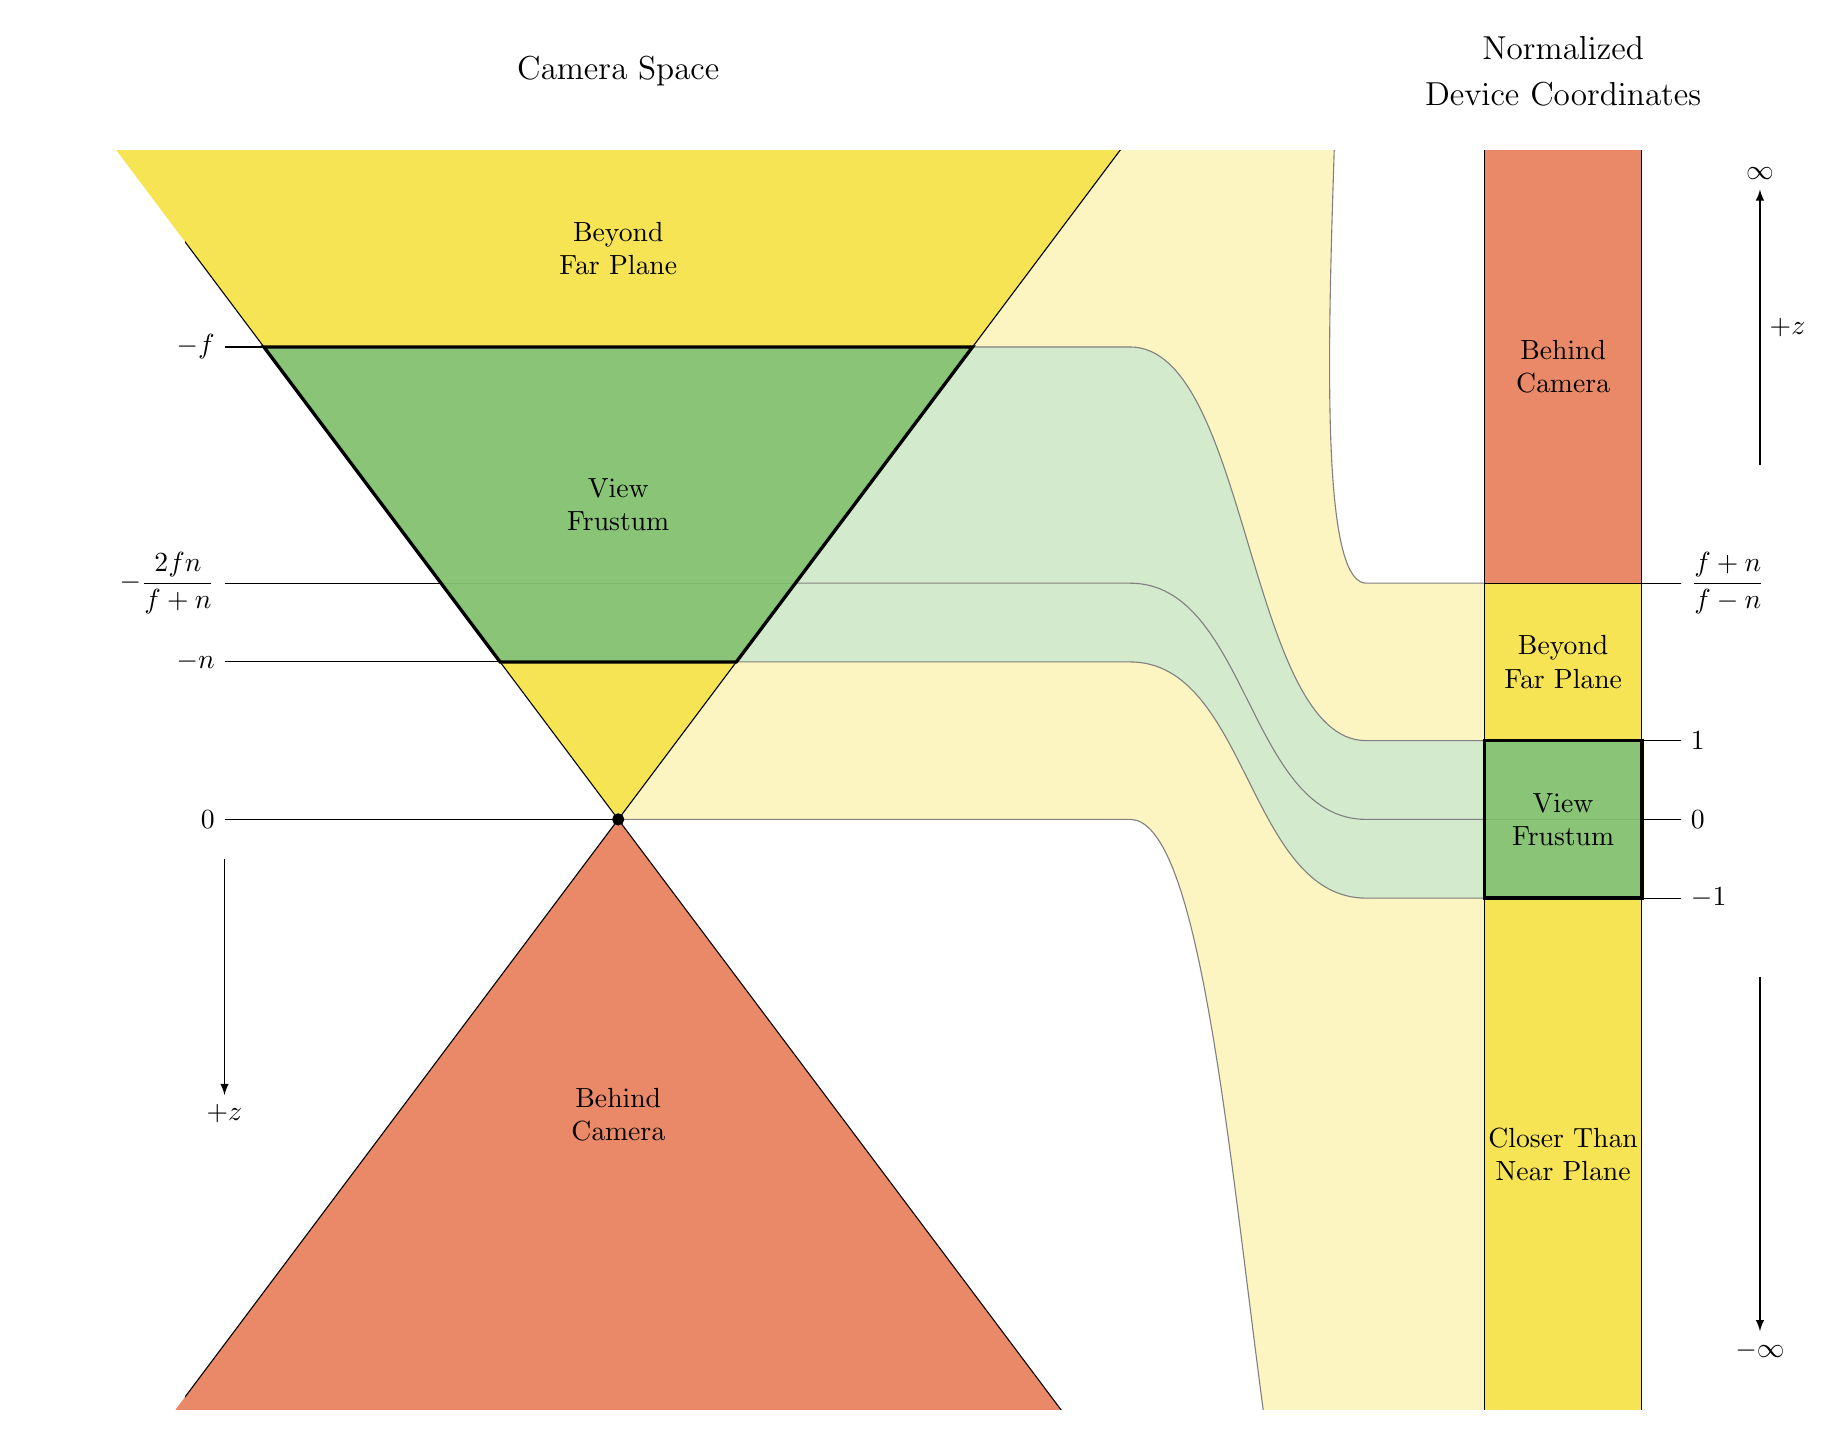
\begin{tikzpicture}[
    font=\rmfamily,
    >=latex
]

\definecolor{vgreen}{HTML}{84C270}
\definecolor{vyellow}{HTML}{F6E34C}
\definecolor{vorange}{HTML}{E8835F}

\begin{scope}
    \clip (-7.5, -7.5) rectangle (13.5, 8.5);

    % ==========================================
    % 1. BACKGROUND FILLS (non-frustum regions only)
    % ==========================================
    
    % Connector fills (behind everything)
    \fill[vyellow, opacity=0.35] 
        (9, 12) .. controls (9.5, 12) and (8.5, 3) .. (9.5, 3) -- (11, 3) --
        (11, 1) -- (9.5, 1) .. controls (8, 1) and (8, 6) .. (6.5, 6) -- (4.5, 6) -- cycle;

    \fill[vgreen, opacity=0.35] 
        (4.5, 6) -- (6.5, 6) .. controls (8, 6) and (8, 1) .. (9.5, 1) -- (11, 1) --
        (11, -1) -- (9.5, -1) .. controls (8, -1) and (8, 2) .. (6.5, 2) -- (1.5, 2) -- cycle;

    \fill[vyellow, opacity=0.35] 
        (1.5, 2) -- (6.5, 2) .. controls (8, 2) and (8, -1) .. (9.5, -1) -- (11, -1) --
        (11, -12) -- (9.5, -12) .. controls (8, -12) and (8, 0) .. (6.5, 0) -- (0, 0) -- cycle;

    % Non-frustum Camera Space fills
    \fill[vorange, opacity=0.95] (0, 0) -- (-9, -12) -- (9, -12) -- cycle;
    \fill[vyellow, opacity=0.95] (0, 0) -- (-1.5, 2) -- (1.5, 2) -- cycle;
    \fill[vyellow, opacity=0.95] (-4.5, 6) -- (-9, 12) -- (9, 12) -- (4.5, 6) -- cycle;

    % Non-frustum NDC Space fills
    \fill[vorange, opacity=0.95] (11, 3) rectangle (13, 12);
    \fill[vyellow, opacity=0.95] (11, 1) rectangle (13, 3);
    \fill[vyellow, opacity=0.95] (11, -12) rectangle (13, -1);

    % ==========================================
    % 2. ANNOTATION LINES & SWOOSHES
    % ==========================================

    % Gray Swooshes 
    \draw[gray, thin] (9, 12) .. controls (9.5, 12) and (8.5, 3) .. (9.5, 3) -- (11, 3);
    \draw[gray, thin] (4.5, 6) -- (6.5, 6) .. controls (8, 6) and (8, 1) .. (9.5, 1) -- (11, 1);
    \draw[gray, thin] (2.25, 3) -- (6.5, 3) .. controls (8, 3) and (8, 0) .. (9.5, 0) -- (11, 0); 
    \draw[gray, thin] (1.5, 2) -- (6.5, 2) .. controls (8, 2) and (8, -1) .. (9.5, -1) -- (11, -1);
    \draw[gray, thin] (0, 0) -- (6.5, 0) .. controls (8, 0) and (8, -12) .. (9.5, -12) -- (11, -12);

    % In the \clip line, change left bound from -7.5 to -5.5:
    \clip (-5.5, -7.5) rectangle (13.5, 8.5);
    
    % Black Lines (Camera Space)
    \draw[thin] (-5, 6) -- (4.5, 6);
    \draw[thin] (-5, 3) -- (2.25, 3);
    \draw[thin] (-5, 2) -- (1.5, 2);
    \draw[thin] (-5, 0) -- (0, 0);

    % Black Lines (NDC Space)
    \draw[thin] (11, 3) -- (14.5, 3);
    \draw[thin] (11, 1) -- (14.5, 1);
    \draw[thin] (11, 0) -- (14.5, 0);
    \draw[thin] (11, -1) -- (14.5, -1);

    % ==========================================
    % 3. FRUSTUM FILLS (drawn after annotation lines to cover them)
    % ==========================================

    \fill[vgreen, opacity=0.95] (-1.5, 2) -- (-4.5, 6) -- (4.5, 6) -- (1.5, 2) -- cycle;
    \fill[vgreen, opacity=0.95] (11, -1) rectangle (13, 1);

    % ==========================================
    % 4. BOX BOUNDARIES & THICK OUTLINES
    % ==========================================
    
    % Camera Space bounds
    \draw[thin] (-9, -12) -- (0, 0) -- (-9, 12); 
    \draw[thin] (9, -12) -- (0, 0) -- (9, 12);   

    % NDC Space bounds (vertical)
    \draw[thin] (11, -12) -- (11, 12);
    \draw[thin] (13, -12) -- (13, 12);

    % Thick Outlines for View Frustum boxes
    \draw[very thick] (-1.5, 2) -- (-4.5, 6) -- (4.5, 6) -- (1.5, 2) -- cycle;
    \draw[very thick] (11, -1) rectangle (13, 1);

    % Focal Point Dot
    \filldraw[black] (0,0) circle (2pt);

\end{scope}

% ==========================================
% 5. LABELS & TEXT
% ==========================================

\node[align=center, font=\large] at (0, 9.5) {Camera Space};
\node[align=center, font=\large] at (12, 9.5) {Normalized\\[0.5ex]Device Coordinates};

\node[align=center] at (0, 7.25) {Beyond\\Far Plane};
\node[align=center] at (0, 4) {View\\Frustum};
\node[align=center] at (0, -3.75) {Behind\\Camera};

\node[align=center] at (12, 5.75) {Behind\\Camera};
\node[align=center] at (12, 2) {Beyond\\Far Plane};
\node[align=center] at (12, 0) {View\\Frustum};
\node[align=center] at (12, -4.25) {Closer Than\\Near Plane};

% ==========================================
% 6. MATH AXES & ARROWS
% ==========================================

\node[left] at (-5, 6) {$-f$};
\node[left] at (-5, 3) {$\displaystyle -\frac{2fn}{f+n}$};
\node[left] at (-5, 2) {$-n$};
\node[left] at (-5, 0) {$0$};

\draw[-latex] (-5, -0.5) -- (-5, -3.5);
\node[below] at (-5, -3.5) {$+z$};

\node[right] at (13.5, 3) {$\displaystyle \frac{f+n}{f-n}$};
\node[right] at (13.5, 1) {$1$};
\node[right] at (13.5, 0) {$0$};
\node[right] at (13.5, -1) {$-1$};

\draw[-latex] (14.5, 4.5) -- (14.5, 8);
\node[above] at (14.5, 8) {$\infty$};
\node[right] at (14.5, 6.25) {$+z$};

\draw[-latex] (14.5, -2) -- (14.5, -6.5);
\node[below] at (14.5, -6.5) {$-\infty$};

\end{tikzpicture}

\end{document}